\chapter{Vector Retrieval}
\label{chapter:flavors}

\abstract{
This chapter sets the stage for the remainder of this monograph.
It explains where vectors come from, how they have come to represent
data of any modality, and why they are a useful mathematical tool in machine learning.
It then describes the structure we typically expect from a collection
of vectors: that similar objects get vector representations that are close to 
each other in an inner product or metric space.
We then define the problem of top-$k$ retrieval over a well-structured
collection of vectors, and explore its different flavors, including
approximate retrieval.
}

\section{Vector Representations}
We routinely use ordered lists of numbers, or \emph{vectors}, to describe objects of any
shape or form. Examples abound. Any geographic location on earth can be recognized as a vector
consisting of its latitude and longitude. A desk can be described as 
a vector that represents its dimensions, area, color, and other quantifiable properties.
A photograph as a list of pixel values that together paint a picture.
A sound wave as a sequence of frequencies.

Vector representations of objects have long been an integral part of the machine learning
literature. Indeed, a classifier, a regression model, or a ranking function learns patterns
from, and acts on, vector representations of data.
In the past, this vector representation of an object was nothing more than
a collection of its \emph{features}.
Every feature described some facet of the object (for example, the color intensity of a pixel
in a photograph) as a continuous or discrete value.
The idea was that, while individual features describe only a small part of the object,
together they provide sufficiently powerful statistics about the object and its properties
for the machine learnt model to act on.

The features that led to the vector representation of an object were generally hand-crafted functions.
To make sense of that, let us consider a text document in English.
Strip the document of grammar and word order, and we end up with a \emph{set} of words,
more commonly known as a ``bag of words.'' This set can be summarized as a histogram.

If we designated every term in the English vocabulary to be
a dimension in a (naturally) high-dimensional space,
then the histogram representation of the document can be encoded as a vector.
The resulting vector has relatively few non-zero coordinates,
and each non-zero coordinate records the frequency of a term present in the document.
This is illustrated in Figure~\ref{figure:flavors:text-sparse-vector} for a toy example.
More generally, non-zero values may be a function of a term's frequency in 
the document and its propensity in a collection---that is, the likelihood of encountering
the term~\citep{salton1988term}.

\begin{figure}[t]
    \centering
    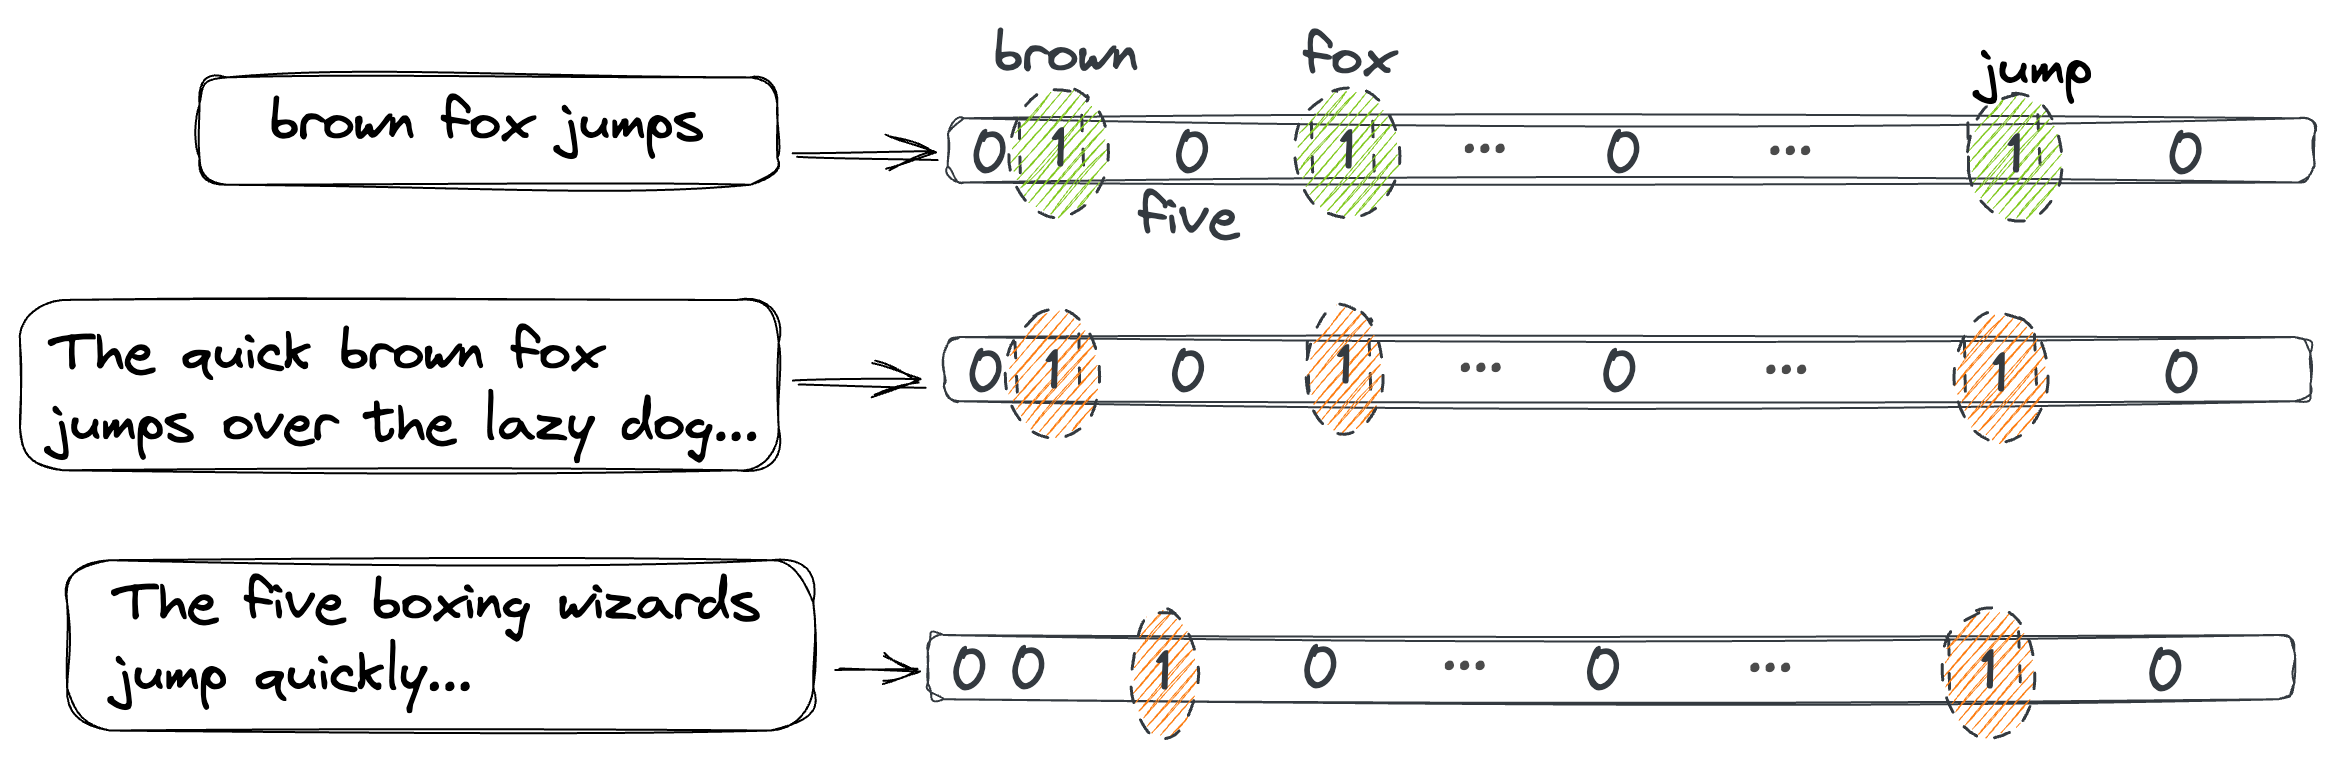
\includegraphics[width=0.8\linewidth]{figures/text-sparse-vector.png}
    \caption{Vector representation of a piece of text by adopting
    a ``bag of words'' view: A text document, when stripped of grammar and word order,
    can be thought of as a vector, where each coordinate represents a term in our vocabulary
    and its value records the frequency of that term in the document or some function of it.
    The resulting vectors are typically \emph{sparse}; that is, they have very few non-zero coordinates.}
    \label{figure:flavors:text-sparse-vector}
\end{figure}

\bigskip

The advent of \emph{deep learning} and, in particular, Transformer-based models~\citep{vaswani2017attention}
brought about vector representations that are beyond the elementary formation above.
The resulting representation is often, as a single entity, referred to as an \emph{embedding},
instead of a ``feature vector,''
though the underlying concept remains unchanged: an object is encoded as a real $d$-dimensional vector,
a point in $\mathbb{R}^d$.

Let us go back to the example from earlier to see how the embedding of a text document
could be different from its representation as a frequency-based feature vector.
Let us maintain the one-to-one mapping between coordinates
and terms in the English vocabulary. Remember that in the ``lexical'' representation from earlier,
if a coordinate was non-zero, that implied that the corresponding term was present in the document
and its value indicated its frequency-based feature. Here we instead \emph{learn} to turn
coordinates on or off and, when we turn a coordinate on, we want its value to predict the
significance of the corresponding term based on semantics and contextual information.
For example, the (absent) synonyms of a (present) term may get a non-zero value, and terms that offer
little discriminative power in the given context become $0$ or close to it.
This basic idea has been explored extensively by many recent models of text~\citep{sparterm,formal2021splade,formal2022splade,zhuang2022reneuir,dai2020sigir,coil,mallia2021learning,zamani2018cikm,unicoil}
and has been shown to produce effective representations.

Vector representations of text need not be sparse.
While sparse vectors with dimensions that are grounded in the vocabulary
are inherently \emph{interpretable}, text documents can also be represented with
lower-dimensional \emph{dense} vectors (where every coordinate is \emph{almost surely} non-zero).
This is, in fact, the most dominant form of vector representation of text
documents in the literature~\citep{lin2021pretrained,karpukhin-etal-2020-dense,xiong2021approximate,reimers-2019-sentence-bert,santhanam-etal-2022-colbertv2,colbert2020khattab}. Researchers have also explored \emph{hybrid}
representations of text where vectors have a dense subspace and an orthogonal sparse
subspace~\citep{chen2022ecir,bruch2023fusion,wang2021bert,Kuzi2020LeveragingSA,karpukhin-etal-2020-dense,Ma2021ARS,Ma2020HybridFR,Wu2019EfficientIP}.

Unsurprisingly, the same embedding paradigm can be extended to other data modalities beyond text:
Using deep learning models, one may embed images, videos, and audio recordings
into vectors. In fact, it is even possible to project different
data modalities (e.g., images and text) together into the same vector space
and preserve some property of interest~\citep{multimodal2020Zhang,guo2019multimodal}.

\begin{svgraybox}
It appears, then, that vectors are everywhere.
Whether they are the result of hand-crafted functions that
capture features of the data or are the output of learnt models;
whether they are dense, sparse, or both,
they are effective representations of data of any modality.
\end{svgraybox}

But what precisely is the point of turning every piece of data into a vector?
One answer to that question takes us to the fascinating world of \emph{retrieval}.

\section{Vectors as Units of Retrieval}

It would make for a vapid exercise if all we had were vector representations of data
without any structure governing a collection of them.
To give a collection of points some structure, we must first ask ourselves what goal
we are trying to achieve by turning objects into vectors.
It turns out, we often intend for the vector representation of two \emph{similar} objects to
be ``close'' to each other according to some well-defined distance function.

That is the structure we desire: Similarity in the vector space must imply similarity
between objects. So, as we engineer features to be extracted from an object, or
design a protocol to learn a model to produce embeddings of data,
we must choose the dimensionality $d$ of the target space
(a subset of $\mathbb{R}^d$) along with a distance function $\delta(\cdot, \cdot)$.
Together, these define an inner product or metric space.

\bigskip

Consider again the lexical representation of a text document
where $d$ is the size of the English vocabulary. Let $\delta$ be the
distance variant of the Jaccard index,
$\delta(u, v) = - J(u, v) \triangleq - \lvert \mathit{nz}(u) \cap \mathit{nz}(v) \rvert / \lvert \mathit{nz}(u) \cup \mathit{nz}(v) \rvert$,
where $\mathit{nz}(u) = \{ i \;|\; u_i \neq 0 \}$ with $u_i$ denoting the $i$-th
coordinate of vector $u$.

In the resulting space, if vectors $u$ and $v$ have a smaller distance
than vectors $u$ and $w$,
then we can clearly conclude that the document represented by $u$ is lexically
more similar to the one represented by $v$ than it is to the document $w$ represents.
That is because the distance (or, in this case, similarity) function reflects
the amount of overlap between the terms present in one document with another.

\bigskip

We should be able to make similar arguments given a semantic embedding of text documents.
Again consider the sparse embeddings with $d$ being the size of the vocabulary,
and more concretely, take \splade{}~\citep{formal2021splade} as a concrete example.
This model produces real-valued sparse vectors in an inner product space.
In other words, the objective of its learning procedure is to
maximize the inner product between similar vectors,
where the inner product between two vectors $u$ and $v$ is
denoted by $\langle u, v \rangle$ and is computed using $\sum_i u_i v_i$.

In the resulting space, if $u$, $v$, and $w$ are generated by \splade{}
with the property that $\langle u, v \rangle > \langle u, w \rangle$, then we can conclude
that, according to \splade{}, documents represented by $u$ and $v$ are semantically more
similar to each other than $u$ is to $w$.
There are numerous other examples of models that optimize for the angular distance
or Euclidean distance ($L_2$) between vectors to preserve (semantic) similarity.

\bigskip

What can we do with a well-characterized collection of vectors that represent real-world
objects? Quite a lot, it turns out. One use case is the topic of this monograph:
the fundamental problem of retrieval.

\begin{svgraybox}
We are often interested in finding $k$ objects that have the highest
degree of similarity to a query object.
When those objects are represented by vectors in a collection $\mathcal{X}$,
where the distance function $\delta(\cdot, \cdot)$ is reflective of similarity,
we may formalize this top-$k$ question mathematically as finding the $k$
minimizers of distance with the query point!
\end{svgraybox}

We state that formally in the following definition:

\begin{definition}[Top-$k$ Retrieval]
\label{definition:flavors:top-k-retrieval}
Given a distance function $\delta(\cdot, \cdot)$, we wish to pre-process
a collection of data points $\mathcal{X} \subset \mathbb{R}^d$
in time that is polynomial in $\lvert \mathcal{X} \rvert$ and $d$,
to form a data structure (the ``index'') whose size is polynomial in
$\lvert \mathcal{X} \rvert$ and $d$, so as to efficiently solve
the following in time $o(\lvert \mathcal{X} \rvert d)$
for an arbitrary query $q \in \mathbb{R}^d$:
\begin{equation}
    \label{equation:flavors:top-k-retrieval}
    \argmin^{(k)}_{u \in \mathcal{X}} \delta(q, u).
\end{equation}
\end{definition}

A web search engine, for example, finds the most relevant documents to your
query by first formulating it as a top-$k$ retrieval problem
over a collection of (not necessarily text-based) vectors.
In this way, it quickly finds the subset of documents from the entire web that
may satisfy the information need captured in your query.
Question answering systems, conversational agents (such as Siri, Alexa, and ChatGPT),
recommendation engines, image search, outlier detectors,
and myriad other applications that are at the forefront
of many online services and in many consumer gadgets
depend on data structures and algorithms that can
answer the top-$k$ retrieval question as efficiently and as effectively as possible.

\section{Flavors of Vector Retrieval}

We create an instance of the deceptively simple
problem formalized in Definition~\ref{definition:flavors:top-k-retrieval}
the moment we acquire a collection of vectors $\mathcal{X}$ together with
a distance function $\delta$.
In the remainder of this monograph, we assume that there is some function,
either manually engineered or learnt, that transforms objects into vectors.
So, from now on, $\mathcal{X}$ is a given.

The distance function then, specifies the flavor of the top-$k$ retrieval problem we need to solve.
We will review these variations and explore what each entails.

\subsection{Nearest Neighbor Search}
In many cases, the distance function is derived from a proper metric
where non-negativity, coincidence, symmetry, and triangle inequality hold for $\delta$.
A clear example of this is the $L_2$ distance:
$\delta(u, v) = \lVert u - v \rVert_2$. The resulting problem,
illustrated for a toy example in Figure~\subref*{figure:flavors:flavors:knn},
is known as $k$-Nearest Neighbors ($k$-NN) search:
\begin{equation}
    \label{equation:flavors:knn}
    \argmin^{(k)}_{u \in \mathcal{X}} \lVert q - u \rVert_2
    = \argmin^{(k)}_{u \in \mathcal{X}} \lVert q - u \rVert_2^2.
\end{equation}

\subsection{Maximum Cosine Similarity Search}

The distance function may also be the angular distance between vectors, which is again a proper metric.
The resulting minimization problem can be stated as follows,
though its equivalent maximization problem (involving the cosine of the angle between
vectors) is perhaps more recognizable:
\begin{equation}
    \label{equation:flavors:kmcs}
    \argmin^{(k)}_{u \in \mathcal{X}} 1 - \frac{\langle q, u \rangle}{\lVert q \rVert_2 \lVert u \rVert_2}
    = \argmax^{(k)}_{u \in \mathcal{X}} \frac{\langle q, u \rangle}{\lVert u \rVert_2}.
\end{equation}
The latter is referred to as the $k$-Maximum Cosine Similarity ($k$-MCS) problem.
Note that, because the norm of the query point, $\lVert q \rVert_2$, is a constant in the
optimization problem, it can simply be discarded; the resulting distance function is
rank-equivalent to the angular distance. Figure~\subref*{figure:flavors:flavors:kmcs}
visualizes this problem on a toy collection of vectors.

\begin{figure}[t]
    \centering
    \subfloat[\textsc{$k$-NN}]{
        \label{figure:flavors:flavors:knn}
        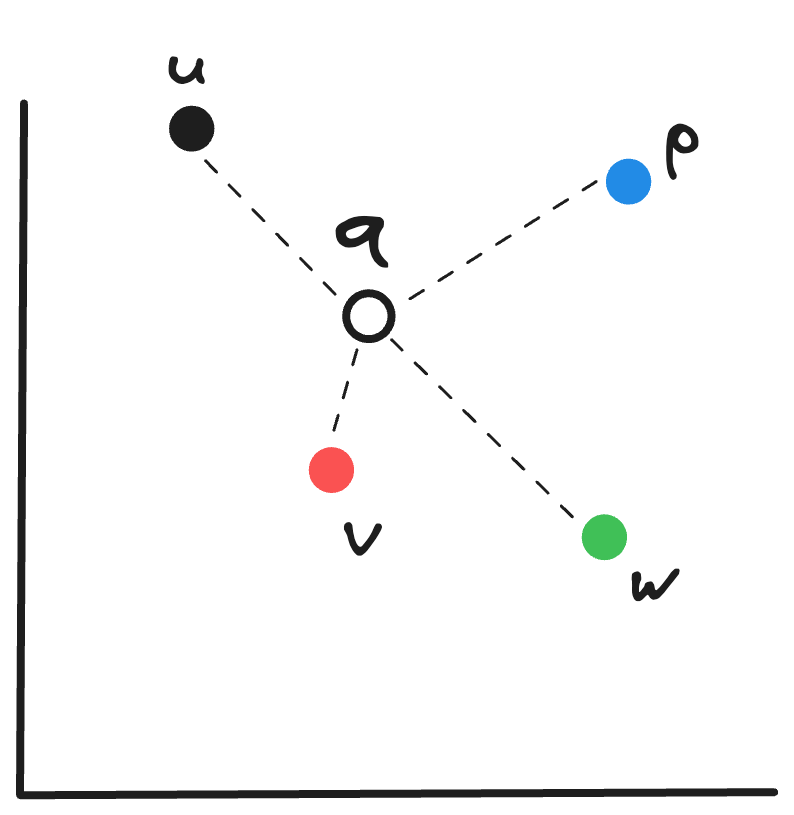
\includegraphics[width=0.32\linewidth]{figures/introduction-l2-knn.png}
    }
    \subfloat[\textsc{$k$-MCS}]{
        \label{figure:flavors:flavors:kmcs}
        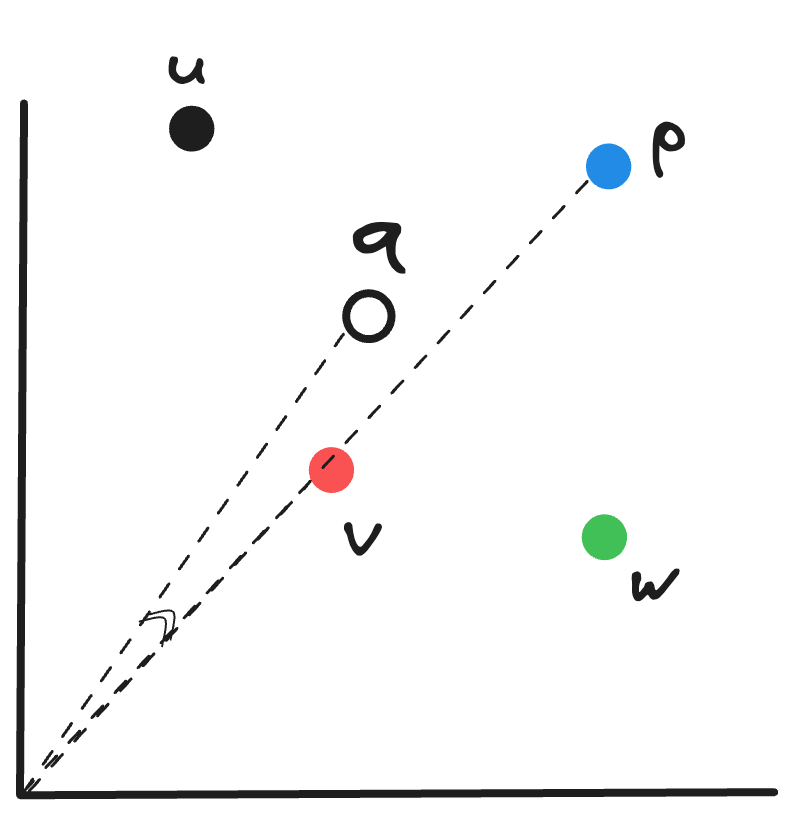
\includegraphics[width=0.32\linewidth]{figures/introduction-kmcs.png}
    }
    \subfloat[\textsc{$k$-MIPS}]{
        \label{figure:flavors:flavors:kmips}
        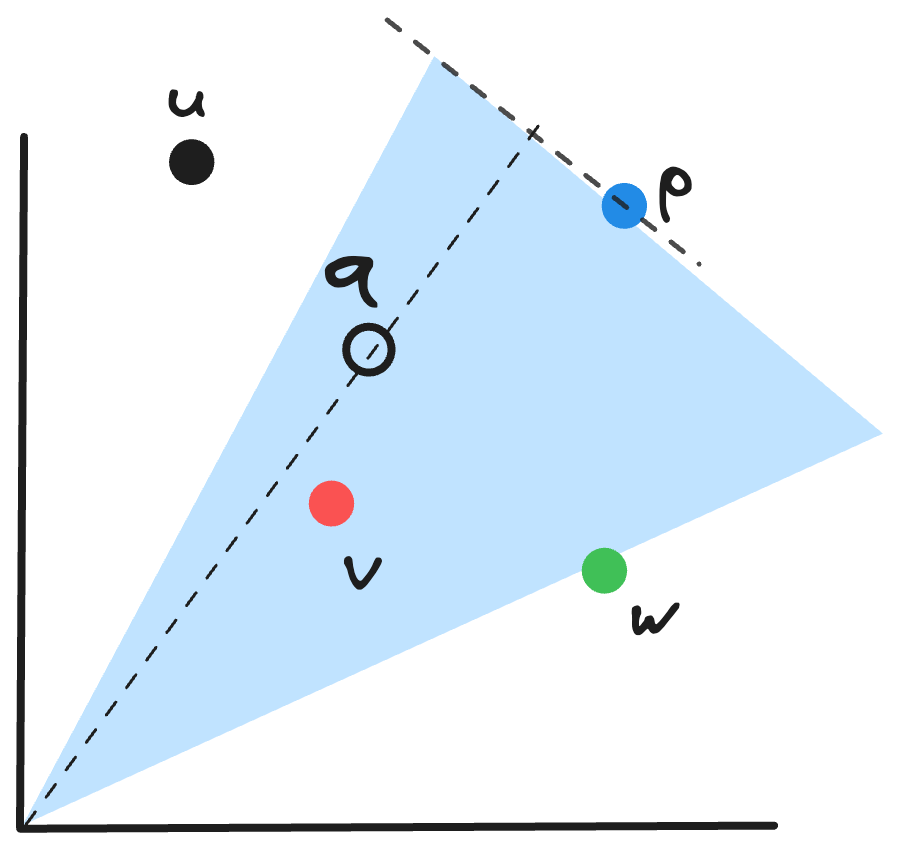
\includegraphics[width=0.32\linewidth]{figures/introduction-kmips.png}
    }
    \caption{Variants of vector retrieval for a toy vector collection in $\mathbb{R}^2$.
    In Nearest Neighbor search, we find the data point whose $L_2$ distance to the
    query point is minimal ($v$ for top-$1$ search). In Maximum Cosine Similarity search, we instead find the point whose
    angular distance to the query point is minimal ($v$ and $p$ are equidistant from the query).
    In Maximum Inner Product Search, we find a vector that maximizes the inner product with the query
    vector. This can be understood as letting the hyperplane orthogonal to the query point sweep the
    space towards the origin; the first vector to touch the sweeping plane is the maximizer of inner product.
    Another interpretation is this: the shaded region in the figure contains all the points $y$
    for which $p$ is the answer to $\argmax_{x \in \{ u, v, w, p\}} \langle x, y \rangle$.}
    \label{figure:flavors:flavors}
\end{figure}

\subsection{Maximum Inner Product Search}
\label{section:flavors:flavors:mips}
Both of the problems in Equations~(\ref{equation:flavors:knn}) and~(\ref{equation:flavors:kmcs})
are special instances of a more general problem known as $k$-Maximum Inner Product Search ($k$-MIPS):
\begin{equation}
    \label{equation:flavors:kmips}
    \argmax^{(k)}_{u \in \mathcal{X}} \langle q, u \rangle.
\end{equation}
This is easy to see for $k$-MCS: If, in a pre-processing step,
we $L_2$-normalized all vectors in $\mathcal{X}$ so that $u$ is transformed to $u^\prime = u / \lVert u \rVert_2$,
then $\lVert u^\prime \rVert_2 = 1$ and therefore Equation~(\ref{equation:flavors:kmcs}) reduces to Equation~(\ref{equation:flavors:kmips}).

As for a reduction of $k$-NN to $k$-MIPS, we can expand Equation~(\ref{equation:flavors:knn})
as follows:
\begin{align*}
    \argmin^{(k)}_{u \in \mathcal{X}} \lVert q - u \rVert_2^2 &=
        \argmin^{(k)}_{u \in \mathcal{X}} \lVert q \rVert_2^2 - 2\langle q, u \rangle + \lVert u \rVert_2^2\\
    &= \argmax^{(k)}_{u^\prime \in \mathcal{X}^\prime} \langle q^\prime, u^\prime \rangle,
\end{align*}
where we have discarded the constant term, $\lVert q \rVert_2^2$,
and defined $q^\prime \in \mathbb{R}^{d+1}$ as the concatenation of $q \in \mathbb{R}^d$ and
a $1$-dimensional vector with value $-1/2$ (i.e., $q^\prime = [q, -1/2]$),
and $u^\prime \in \mathbb{R}^{d+1}$ as $[u, \lVert u \rVert_2^2]$.

The $k$-MIPS problem, illustrated on a toy collection in
Figure~\subref*{figure:flavors:flavors:kmips}, does not come about just as the result of the reductions
shown above. In fact, there exist embedding models (such as \splade{}, as discussed earlier)
that learn vector representations with respect to inner product as the distance function.
In other words, $k$-MIPS is an important problem in its own right.

\subsubsection{Properties of MIPS}

In a sense, then, it is sufficient to solve the $k$-MIPS problem
as it is the umbrella problem for much of vector retrieval.
Unfortunately, $k$-MIPS is a much harder problem than the other variants.
That is because inner product is not a proper metric.
In particular, it is not non-negative and does not satisfy the triangle inequality, so that
$\langle u, v \rangle \nless \langle u, w \rangle + \langle w, v \rangle$ in general.

\begin{svgraybox}
Perhaps more troubling is the fact that even ``coincidence'' is not guaranteed.
In other words, it is not true in general that a vector $u$ maximizes
inner product with itself: $u \neq \argmax_{v \in \mathcal{X}} \langle v, u \rangle$!
\end{svgraybox}

As an example, suppose $v$ and $p = \alpha v$ for some $\alpha > 1$ are vectors
in the collection $\mathcal{X}$---a case demonstrated in Figure~\subref*{figure:flavors:flavors:kmips}.
Clearly, we have that $\langle v, p \rangle = \alpha \langle v, v \rangle > \langle v, v \rangle$,
so that $p$ (and not $v$) is the solution to MIPS\footnote{When $k=1$, we drop the symbol $k$ from the name of the retrieval problem. So we write MIPS instead of $1$-MIPS.}
for the query point $v$.

In high-enough dimensions and under certain statistical conditions, however,
coincidence is reinstated for MIPS with high probability. One such case is stated in the 
following theorem.

\begin{theorem}
    \label{theorem:flavors:coincidence}
    Suppose data points $\mathcal{X}$ are independent and identically distributed (\emph{iid}) in each dimension
    and drawn from a zero-mean distribution. Then, for any $u \in \mathcal{X}$:
    \begin{equation*}
        \lim_{d \rightarrow \infty} \probability\big[ u = \argmax_{v \in \mathcal{X}}  \langle u, v \rangle ] = 1.
    \end{equation*}
\end{theorem}
\begin{proof}
    Denote by $\var[\cdot]$ and $\ev[\cdot]$ the variance and expected value operators.
    By the conditions of the theorem, it is clear that $\ev[\langle u, u \rangle] = d \ev[Z^2]$ where
    $Z$ is the random variable that generates each coordinate of the vector. We can also see that
    $\ev[\langle u, X \rangle] = 0$ for a random data point $X$, and that
    $\var[\langle u, X \rangle] = \lVert u \rVert_2^2 \ev[Z^2]$.

    We wish to claim that $u \in \mathcal{X}$ is the solution to a MIPS problem where $u$ is also the query point.
    That happens if and only if every other vector in $\mathcal{X}$ has an inner product with $u$ that is smaller than
    $\langle u, u\rangle$. So that:
    \begin{align*}
        \probability\big[ u &= \argmax_{v \in \mathcal{X}}  \langle u, v \rangle ] =
            \probability\big[ \langle u, v \rangle \leq \langle u, u \rangle \quad \forall \; v \in \mathcal{X} ] = \\
            &1 - \probability\big[ \exists \; v \in \mathcal{X} \; \mathit{s.t.} \quad \langle u, v \rangle > \langle u, u \rangle] \geq && \text{(by Union Bound)} \\
            &1 - \sum_{v \in \mathcal{X}} \probability\big[ \langle u, v \rangle > \langle u, u \rangle] = && \text{(by \emph{iid})} \\
            &1 - \lvert \mathcal{X} \rvert \probability\big[ \langle u, X \rangle > \langle u, u \rangle].
    \end{align*}
    Let us turn to the last term and bound the probability for a random data point:
    \begin{equation*}
        \probability\big[\langle u, X \rangle > \langle u, u \rangle] =
        \probability\big[ \underbrace{\langle u, X \rangle - \langle u, u \rangle + d \ev[Z^2]}_{Y} > d \ev[Z^2] \big].
    \end{equation*}
    The expected value of $Y$ is $0$. Denote by $\sigma^2$ its variance. By the application of the one-sided
    Chebyshev's inequality,\footnote{The one-sided Chebyshev's inequality for a random variable $X$ with
    mean $\mu$ and variance $\sigma^2$ states that $\probability\big[ X - \mu > t\big] \leq \sigma^2 / \big( \sigma^2 + t^2 \big)$.}
    we arrive at the following bound:
    \begin{equation*}
        \probability\big[\langle u, X \rangle > \langle u, u \rangle] \leq \frac{\sigma^2}{\sigma^2 + d^2 \ev[Z^2]^2}.
    \end{equation*}
    Note that, $\sigma^2$ is a function of the sum of \emph{iid} random variables, and, as such, grows linearly with $d$.
    In the limit. this probability tends to $0$. We have thus shown that
    $\lim_{d \rightarrow \infty} \probability\big[ u = \argmax_{v \in \mathcal{X}}  \langle u, v \rangle ] \geq 1$ which concludes
    the proof.
\end{proof}

\begin{figure}[t]
    \centering
    \subfloat[\textsc{Synthetic}]{
        \label{figure:flavors:coincidence:synthetic}
        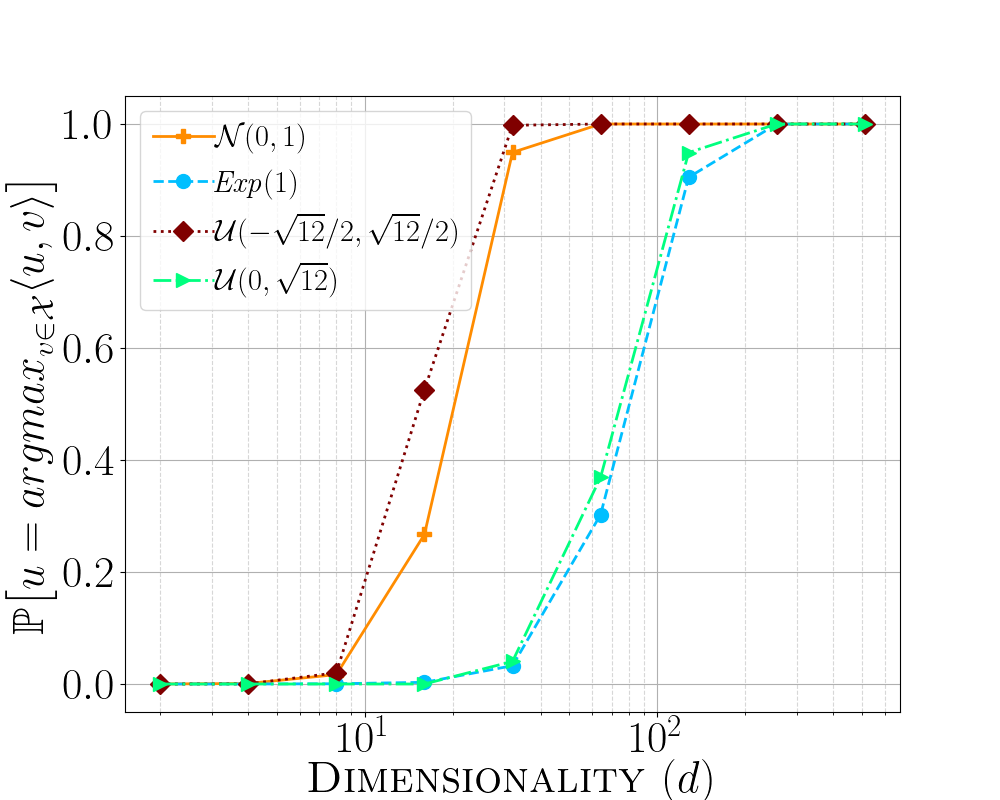
\includegraphics[width=0.52\linewidth]{figures/introduction-coincidence-synthetic.png}
    }\hspace*{-1.5em}
    \subfloat[\textsc{Real}]{
        \label{figure:flavors:coincidence:real}
        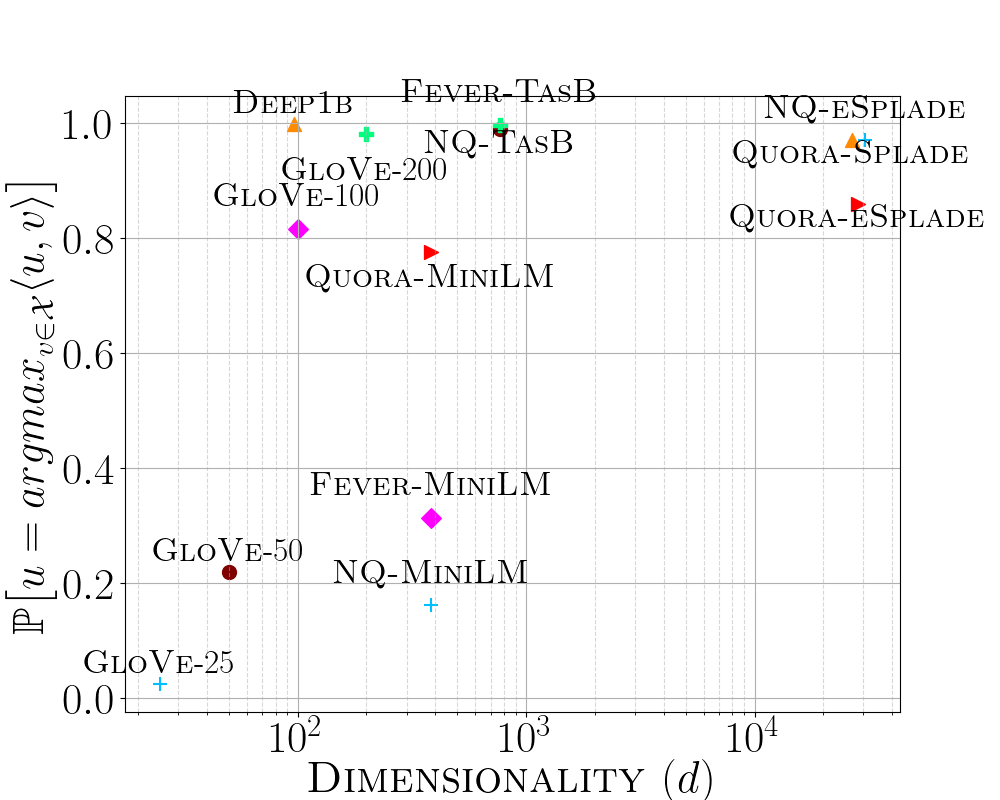
\includegraphics[width=0.52\linewidth]{figures/introduction-coincidence-real.png}
    }
    \caption{Probability that $u \in \mathcal{X}$ is the solution to MIPS over $\mathcal{X}$ with query $u$
    versus the dimensionality $d$, for various synthetic and real collections $\mathcal{X}$.
    For synthetic collections, $\lvert \mathcal{X} \rvert = 100{,}000$. Appendix~\ref{appendix:collections}
    gives a description of the real collections. Note that, for real collections, we estimate the reported
    probability by sampling $10{,}000$ data points and using them as queries. Furthermore,
    we do not pre-process the vectors---importantly, we do not $L_2$-normalize the collections.}
    \label{figure:flavors:coincidence}
\end{figure}

\subsubsection{Empirical Demonstration of the Lack of Coincidence}
Let us demonstrate the effect of Theorem~\ref{theorem:flavors:coincidence}
empirically. First, let us choose distributions that meet
the requirements of the theorem: a Gaussian distribution
with mean $0$ and variance $1$, and a uniform distribution over $[-\sqrt{12}/2, \sqrt{12}/2]$
(with variance $1$) will do.
For comparison, choose another set of distributions that do not have the requisite properties:
Exponential with rate $1$ and uniform over $[0, \sqrt{12}]$.
Having fixed the distributions, we next sample $100{,}000$ random vectors
from them to form a collection $\mathcal{X}$.
We then take each data point, use it as a query in MIPS over $\mathcal{X}$, and
report the proportion of data points that are solutions to their own search.

Figure~\subref*{figure:flavors:coincidence:synthetic} illustrates the results of this experiment.
As expected, for the Gaussian and centered uniform distributions, the ratio of interest approaches $1$
when $d$ is sufficiently large. Surprisingly, even when the distributions do not strictly satisfy
the conditions of the theorem, we still observe the convergence of that ratio to $1$. So it appears that
the requirements of Theorem~\ref{theorem:flavors:coincidence} are more forgiving than one may imagine.

We also repeat the exercise above on several real-world collections, a description of which
can be found in Appendix~\ref{appendix:collections} along with salient statistics.
The results of these experiments are visualized in Figure~\subref*{figure:flavors:coincidence:real}.
As expected, whether a data point maximizes inner product with itself entirely depends
on the underlying data distribution. We can observe that, for some collections
in high dimensions, we are likely to encounter coincidence in the sense we defined
earlier, but for others that is clearly not the case. It is important to keep this
difference between synthetic and real collections in mind when designing experiments
that evaluate the performance of MIPS systems.

\section{Approximate Vector Retrieval}
\label{chapter:flavors:approximate}

Saying one problem is harder than another neither implies that we cannot approach
the harder problem, nor does it mean that the ``easier'' problem is easy to solve.
In fact, none of these variants of vector retrieval ($k$-NN, $k$-MCS, and $k$-MIPS)
can be solved exactly \emph{and} efficiently in high dimensions.
Instead, we must either accept that the solution would be inefficient
(in terms of space- or time-complexity), or allow some degree of error.

\begin{figure}[t]
    \centering
    \subfloat[\textsc{$k$-NN}]{
        \label{figure:flavors:flavors:approximate-knn}
        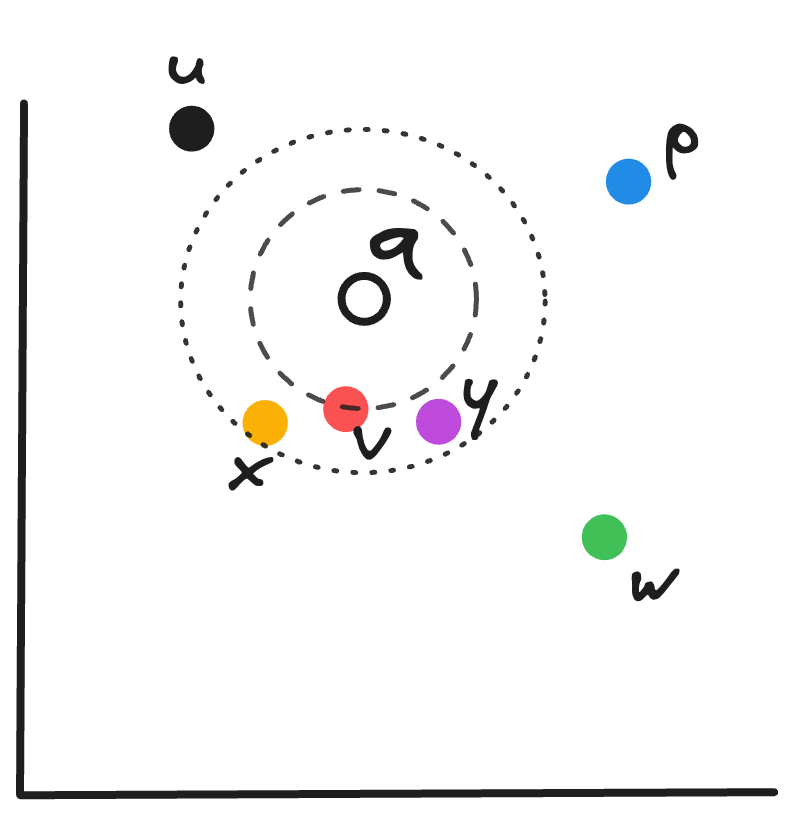
\includegraphics[width=0.32\linewidth]{figures/introduction-approximate-l2-knn.png}
    }
    \subfloat[\textsc{$k$-MCS}]{
        \label{figure:flavors:flavors:approximate-kmcs}
        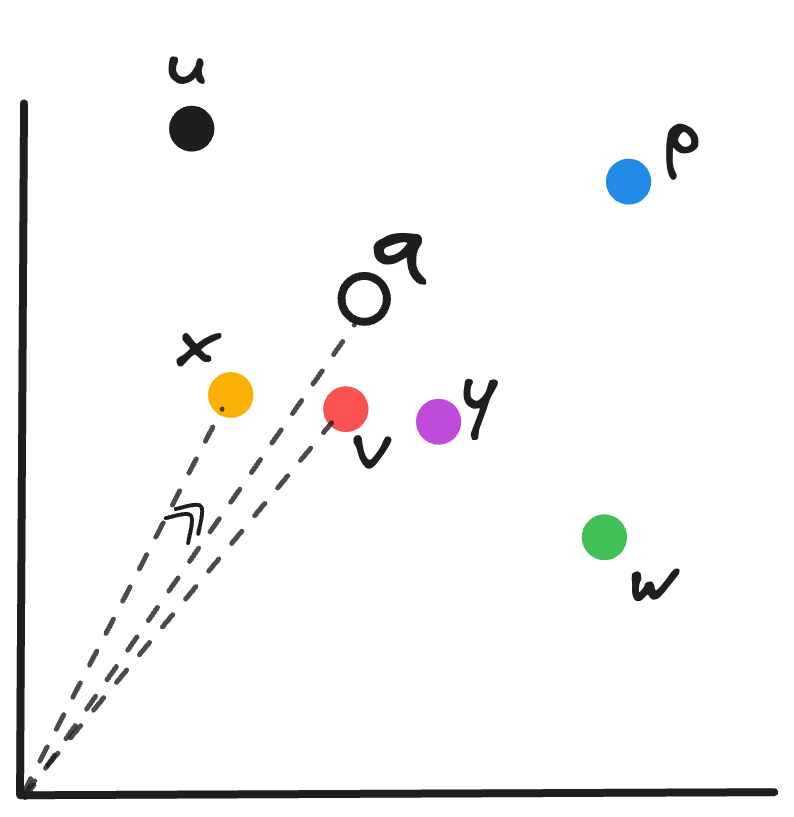
\includegraphics[width=0.32\linewidth]{figures/introduction-approximate-kmcs.png}
    }
    \subfloat[\textsc{$k$-MIPS}]{
        \label{figure:flavors:flavors:approximate-kmips}
        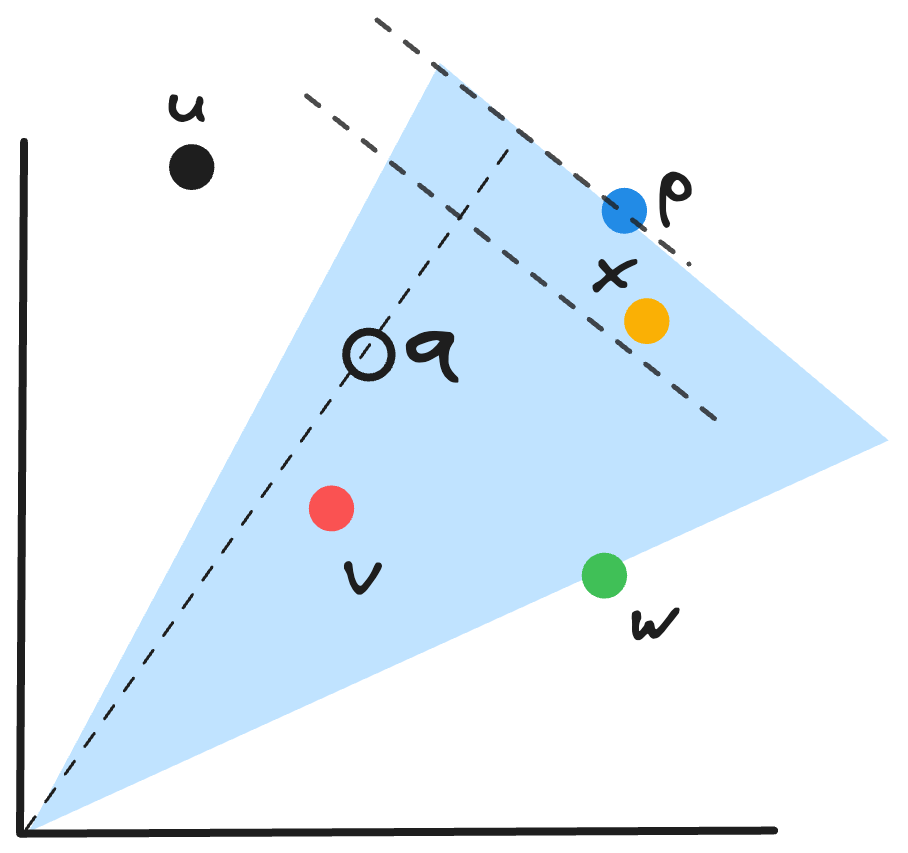
\includegraphics[width=0.32\linewidth]{figures/introduction-approximate-kmips.png}
    }
    \caption{Approximate variants of top-$1$ retrieval for a toy collection in $\mathbb{R}^2$.
    In NN, we admit vectors that are at most $\epsilon$ away from the optimal solution. As such,
    $x$ and $y$ are both valid solutions as they are in a ball with radius $(1+\epsilon) \delta(q, x)$
    centered at the query.
    Similarly, in MCS, we accept a vector (e.g., $x$) if its angle with the query point is at most $1 + \epsilon$
    greater than the angle between the query and the optimal vector (i.e., $v$).
    For the MIPS example, assuming that the inner product of query and $x$ is at most
    $(1 - \epsilon)$-times the inner product of query and $p$, then $x$ is an acceptable solution.}
    \label{figure:flavors:flavors-approximate}
\end{figure}

The first case of solving the problem exactly but inefficiently is uninteresting: If we are looking
to find the solution for $k=1$, for example, it is enough to compute the distance function
for every vector in the collection and the query, resulting in linear complexity.
When $k > 1$, the total time complexity is $\mathcal{O}(\lvert \mathcal{X} \rvert d \log k)$,
where $\lvert \mathcal{X} \rvert$ is the size of the collection.
So it typically makes more sense to investigate the second strategy of admitting error.

That argument leads naturally to the class of $\epsilon$-\emph{approximate} vector retrieval problems.
This idea can be formalized rather easily for the special case where $k=1$:
The approximate solution for the top-$1$ retrieval is satisfactory so long as the vector $u$
returned by the algorithm is at most $(1 + \epsilon)$ factor farther than the
optimal vector $u^\ast$, according to $\delta(\cdot, \cdot)$ and for some arbitrary
$\epsilon > 0$:
\begin{equation}
    \label{equation:flavors:approximate-top-k-retrieval}
    \delta(q, u) \leq (1 + \epsilon) \delta(q, u^\ast).
\end{equation}
Figure~\ref{figure:flavors:flavors-approximate} renders the solution space for
an example collection in $\mathbb{R}^2$.

The formalism above extends to the more general case where $k > 1$ in an obvious way:
a vector $u$ is a valid solution to the $\epsilon$-approximate top-$k$ problem if its distance
to the query point is at most $(1 + \epsilon)$ times the distance to the $k$-th
optimal vector. This is summarized in the following definition:

\begin{definition}[$\epsilon$-Approximate Top-$k$ Retrieval]
\label{definition:flavors:approximate-top-k-retrieval}
Given a distance function $\delta(\cdot, \cdot)$, we wish to pre-process
a collection of data points $\mathcal{X} \subset \mathbb{R}^d$
in time that is polynomial in $\lvert \mathcal{X} \rvert$ and $d$,
to form a data structure (the ``index'') whose size is polynomial in
$\lvert \mathcal{X} \rvert$ and $d$, so as to efficiently solve
the following in time $o(\lvert \mathcal{X} \rvert d)$
for an arbitrary query $q \in \mathbb{R}^d$ and $\epsilon > 0$:
\begin{equation*}
    \mathcal{S} =\argmin^{(k)}_{u \in \mathcal{X}}  \delta(q, u),
\end{equation*}
such that for all $u \in \mathcal{S}$,
Equation~(\ref{equation:flavors:approximate-top-k-retrieval}) is satisfied
where $u^\ast$ is the $k$-th optimal vector obtained by solving the problem
in Definition~\ref{definition:flavors:top-k-retrieval}.
\end{definition}

Despite the extension to top-$k$ above, it is more common
to characterize the effectiveness of an approximate top-$k$ solution
as the percentage of correct vectors that are present in the solution. Concretely,
if $\mathcal{S} = \argmax^{(k)}_{u \in \mathcal{X}} \delta(q, u)$ is the exact set of top-$k$ vectors,
and $\tilde{\mathcal{S}}$ is the approximate set, then the \emph{accuracy} of the approximate algorithm
can be reported as $\lvert \mathcal{S} \cap \tilde{\mathcal{S}} \rvert / k$.\footnote{
This quantity is also known as \emph{recall} in the literature, because we
are counting the number of vectors our algorithm recalls from the exact solution set.}

This monograph primarily studies the approximate\footnote{
We drop $\epsilon$ from the name when it is clear from context.} retrieval problem.
As such, while we state a retrieval problem using the $\argmax$ or $\argmin$
notation, we are generally only interested in approximate solutions to it.

\bibliographystyle{abbrvnat}
\bibliography{biblio}
